% Options for packages loaded elsewhere
\PassOptionsToPackage{unicode}{hyperref}
\PassOptionsToPackage{hyphens}{url}
%
\documentclass[
]{article}
\usepackage{amsmath,amssymb}
\usepackage{lmodern}
\usepackage{iftex}
\ifPDFTeX
  \usepackage[T1]{fontenc}
  \usepackage[utf8]{inputenc}
  \usepackage{textcomp} % provide euro and other symbols
\else % if luatex or xetex
  \usepackage{unicode-math}
  \defaultfontfeatures{Scale=MatchLowercase}
  \defaultfontfeatures[\rmfamily]{Ligatures=TeX,Scale=1}
\fi
% Use upquote if available, for straight quotes in verbatim environments
\IfFileExists{upquote.sty}{\usepackage{upquote}}{}
\IfFileExists{microtype.sty}{% use microtype if available
  \usepackage[]{microtype}
  \UseMicrotypeSet[protrusion]{basicmath} % disable protrusion for tt fonts
}{}
\makeatletter
\@ifundefined{KOMAClassName}{% if non-KOMA class
  \IfFileExists{parskip.sty}{%
    \usepackage{parskip}
  }{% else
    \setlength{\parindent}{0pt}
    \setlength{\parskip}{6pt plus 2pt minus 1pt}}
}{% if KOMA class
  \KOMAoptions{parskip=half}}
\makeatother
\usepackage{xcolor}
\usepackage[margin=1in]{geometry}
\usepackage{graphicx}
\makeatletter
\def\maxwidth{\ifdim\Gin@nat@width>\linewidth\linewidth\else\Gin@nat@width\fi}
\def\maxheight{\ifdim\Gin@nat@height>\textheight\textheight\else\Gin@nat@height\fi}
\makeatother
% Scale images if necessary, so that they will not overflow the page
% margins by default, and it is still possible to overwrite the defaults
% using explicit options in \includegraphics[width, height, ...]{}
\setkeys{Gin}{width=\maxwidth,height=\maxheight,keepaspectratio}
% Set default figure placement to htbp
\makeatletter
\def\fps@figure{htbp}
\makeatother
\setlength{\emergencystretch}{3em} % prevent overfull lines
\providecommand{\tightlist}{%
  \setlength{\itemsep}{0pt}\setlength{\parskip}{0pt}}
\setcounter{secnumdepth}{-\maxdimen} % remove section numbering
\usepackage{booktabs}
\usepackage{longtable}
\usepackage{array}
\usepackage{multirow}
\usepackage{wrapfig}
\usepackage{float}
\usepackage{colortbl}
\usepackage{pdflscape}
\usepackage{tabu}
\usepackage{threeparttable}
\usepackage{threeparttablex}
\usepackage[normalem]{ulem}
\usepackage{makecell}
\usepackage{xcolor}
\ifLuaTeX
  \usepackage{selnolig}  % disable illegal ligatures
\fi
\IfFileExists{bookmark.sty}{\usepackage{bookmark}}{\usepackage{hyperref}}
\IfFileExists{xurl.sty}{\usepackage{xurl}}{} % add URL line breaks if available
\urlstyle{same} % disable monospaced font for URLs
\hypersetup{
  pdftitle={Supplementary data - Phonological Networks and Systematicity in Early Lexical Acquisition},
  pdfauthor={anonymised for review},
  hidelinks,
  pdfcreator={LaTeX via pandoc}}

\title{Supplementary data - Phonological Networks and Systematicity in
Early Lexical Acquisition}
\author{anonymised for review}
\date{}

\begin{document}
\maketitle

\hypertarget{s1-age-of-production-aop-connectivity}{%
\subsubsection{S1: Age of production (AoP) \textasciitilde{}
connectivity}\label{s1-age-of-production-aop-connectivity}}

\begin{longtable}[t]{cccc}
\caption{\label{tab:table-aop-deg-corr}S1: Outputs (rho and p values) of AoP ~ degree Spearman's correlation tests for each infant in the dataset.}\\
\toprule
Speaker & Corpus & rho & p\\
\midrule
Alex & English & -0.20 & <0.001\\
Lily & English & -0.25 & <0.001\\
Naima & English & -0.28 & <0.001\\
Violet & English & -0.26 & <0.001\\
William & English & -0.22 & <0.001\\
\addlinespace
Anais & French & -0.02 & 0.593\\
Marie & French & -0.18 & <0.001\\
Nathan & French & -0.11 & 0.045\\
Tim & French & -0.21 & <0.001\\
\bottomrule
\end{longtable}

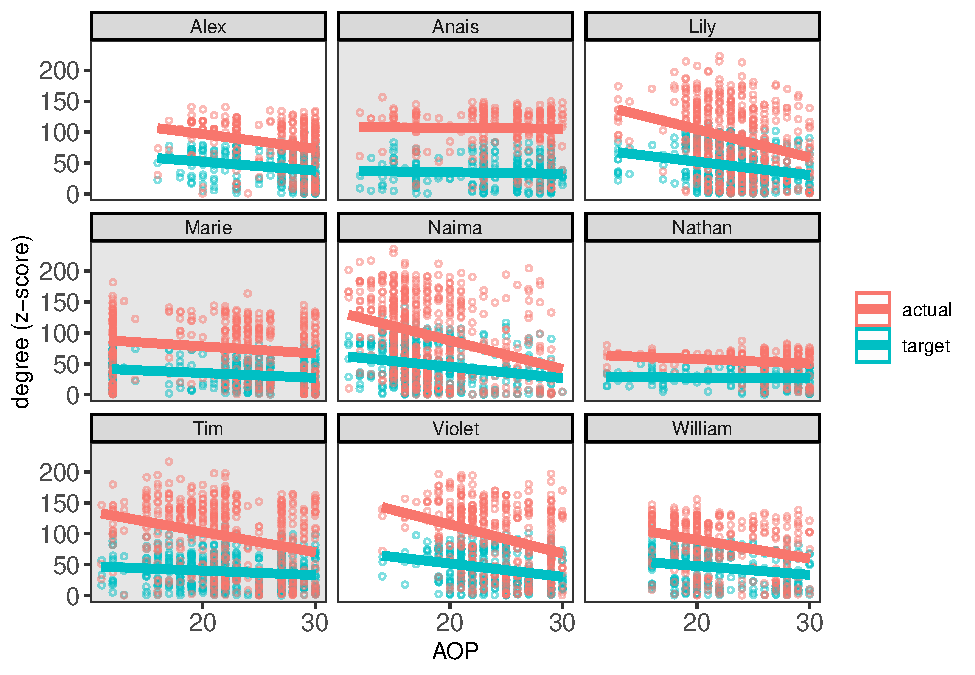
\includegraphics{PhonNetworksSupplementaryData-anon_files/figure-latex/Figure-AOP-deg-corr-1.pdf}
\newpage

\hypertarget{s2-network-growth-models-full-model-outputs}{%
\subsubsection{S2: Network growth models: Full model
outputs}\label{s2-network-growth-models-full-model-outputs}}

\begin{longtable}[t]{ccccccccc}
\caption{\label{tab:full-data-summary}Full results from maximal logistic regression model (model 3) testing the effects of network growth values, corpus (English as baseline), word frequency and word length to predict word acquisition. All variables were scaled and centred. Word category was defined according to word categories on the McArthur Bates CDI (Fenson et al., 1994)}\\
\toprule
\multicolumn{1}{c}{ } & \multicolumn{4}{c}{Actual} & \multicolumn{4}{c}{Target} \\
\cmidrule(l{3pt}r{3pt}){2-5} \cmidrule(l{3pt}r{3pt}){6-9}
Effect & beta & SE & z & p & beta & SE & z & p\\
\midrule
Intercept & -2.88 & 0.16 & -17.80 & <0.001 & -3.00 & 0.18 & -16.96 & <0.001\\
Length & -0.21 & 0.04 & -4.73 & <0.001 & -0.22 & 0.05 & -4.77 & <0.001\\
Age & 1.04 & 0.12 & 8.93 & <0.001 & 1.11 & 0.11 & 10.35 & <0.001\\
n Tokens & 0.60 & 0.04 & 16.35 & <0.001 & 0.62 & 0.04 & 16.61 & <0.001\\
Word frequency & -0.03 & 0.03 & -1.06 & 0.287 & -0.04 & 0.03 & -1.27 & 0.205\\
\addlinespace
Corpus & 0.40 & 0.10 & 4.00 & <0.001 & 0.68 & 0.14 & 4.74 & <0.001\\
Categoryverbs & -0.46 & 0.05 & -8.34 & <0.001 & -0.44 & 0.06 & -7.97 & <0.001\\
Category: connecting words & -0.62 & 0.21 & -2.94 & 0.003 & -0.63 & 0.21 & -2.99 & 0.003\\
Category: adjectives & -0.18 & 0.08 & -2.21 & 0.027 & -0.19 & 0.08 & -2.30 & 0.021\\
Category: games/routines & 0.14 & 0.14 & 1.02 & 0.310 & 0.15 & 0.14 & 1.02 & 0.306\\
\addlinespace
Category: prepositions & -0.37 & 0.20 & -1.90 & 0.057 & -0.37 & 0.20 & -1.89 & 0.059\\
Category: pronouns & -0.29 & 0.12 & -2.39 & 0.017 & -0.28 & 0.12 & -2.31 & 0.021\\
Category: quantifiers & -0.33 & 0.15 & -2.23 & 0.026 & -0.36 & 0.15 & -2.46 & 0.014\\
Category: question words & -0.95 & 0.24 & -3.92 & <0.001 & -0.95 & 0.25 & -3.86 & <0.001\\
Category: onomatopoeia & 0.74 & 0.16 & 4.67 & <0.001 & 0.75 & 0.16 & 4.69 & <0.001\\
\addlinespace
Category: time & -0.50 & 0.21 & -2.34 & 0.019 & -0.48 & 0.21 & -2.22 & 0.026\\
Category: locations & -0.04 & 0.15 & -0.25 & 0.802 & -0.03 & 0.16 & -0.16 & 0.869\\
PAQ value & 0.06 & 0.04 & 1.52 & 0.127 & 0.08 & 0.04 & 1.97 & 0.049\\
PAT value & 0.29 & 0.05 & 6.35 & <0.001 & 0.30 & 0.06 & 4.75 & <0.001\\
Age x Length & 0.15 & 0.04 & 4.23 & <0.001 & 0.14 & 0.04 & 3.95 & <0.001\\
\addlinespace
Age x n Tokens & 0.28 & 0.03 & 8.74 & <0.001 & 0.30 & 0.03 & 9.10 & <0.001\\
Age x Frequency & 0.11 & 0.03 & 3.72 & <0.001 & 0.12 & 0.03 & 3.82 & <0.001\\
Age x PAQ & 0.03 & 0.03 & 0.90 & 0.370 & 0.00 & 0.03 & 0.03 & 0.980\\
Age x PAT & -0.03 & 0.02 & -1.70 & 0.089 & -0.01 & 0.03 & -0.37 & 0.713\\
\bottomrule
\end{longtable}

\end{document}
